\chapter{Analysis}\label{chap:analysis}
    In this chapter, the general problem area of the danish people's concern about climate change, or the lack thereof, will be described. An apparent inconsistency between climate change awareness and the personal climate actions will also be investigated. Furthermore, the potential of narrative games, particularly in  Immersive Virtual Reality(VR), as an approach for affecting real life behaviour, will be explored. The knowledge obtained throughout this chapter, will culminate in a set of design requirements and a problem statement that will be used to design, develop and evaluate upon a prototype of a VR game with personal climate actions as the main theme.

\section{Problem Area}\label{sec:problemArea}
    For several years the consensus among scientists and the reliability of the scientific data regarding anthropogenic climate change, and predictions about future impact, has increased, making the issue hard to deny\cite{the5Ds, scientistConsensus, publicEngagementUnderstanding}. Around one third of many countries' carbon emission come from domestic energy-use and private travel\cite{reorientingClimageChangeCommunication}. There is, however, still a discrepancy between the public's awareness of the subject, in developed countries such as Denmark, and what individual people do to reduce their personal carbon footprint. Most of these people's lack of personal climate action, is a result of a psychological distancing towards the matter\cite{the5Ds, publicEngagementUnderstanding}. They believe that there will be no immediate personal consequences, because climate change is both spatially and temporally far away\cite{publicEngagementUnderstanding}.
    
    \subsection{Climate survey}
        In a survey from 2018, made by the danish think tank Concito\footnote{\href{https://concito.dk}{Concito Website: https://concito.dk}}, respondents(n=1076) were asked about their opinions on climate change and their personal ${CO_2}$ footprint.
        
        The respondents were asked about how serious climate change was on a global scale. 46\% and 42\% responded with either very serious or to some degree, respectively. 
        
        Mostly, the Danes were concerned about more extreme storms and downpours (73\%), rising water levels (65\%), larger and more widespread desert areas (59\%), increasing extinction of animal and plant species (55\%), and increased lack of drinkable water (52\%). The question accepted multiple answers\cite{concito}.
        % There is an awareness and a global concern
        
        When asked about to what degree they themselves were feeling the effects of climate changes, 4\% said that they were experiencing it to a great extent, while 21\% replied only to some extent. This leaves 44\% saying that they experienced it to a lesser degree and 24\% replying they did not experience at all\cite{concito}. This correlates with another question of the survey asking about how concerned the respondent were that climate change would personally hurt them, where 11\% said that they were greatly worried about damage to them, and 37\% replied that they were to some extent worried\cite{concito}.
        % Do not feel the effects
        
        When asked, 54\% said that they believe it is necessary for them to make behavioural lifestyle changes, while 24\% believe that technology will solve the climate issues, without them needing to make substantial lifestyle changes\cite{concito}.
        % About half feel a personal responsibility
        
        The danish people believe the strongest individual counter measure in order to reduce their personal carbon emission to be garbage sorting (38\%), riding the bike or public transportation (32\%), replacing their current car with an electric or hybrid version (31\%), and flying less (30\%). The question accepted a maximum of 5 answers\cite{concito}.
        % Believe in mostly transportation related solutions

        When it comes down to the expected climate action, the individual Dane does not make the required sacrifices to live up to their own expectations, with only 16\% saying they flew less from 2016-2018 and less than half(48\%) use the bike or public transportation. The question accepted multiple answers\cite{concito}.
        % People still fly a lot knowing that it is a "sin" only some people use bike or public transportation
        
        When asked about motives for making an effort towards more climate friendly measures like using public transport instead of a car, insulating their house post build, or buying less energy intensive appliances, only 30\% said that they did it to help the environment, while 31\% said they did it to save money. 23\% did however reply that they simply did not do those environmentally friendly efforts\cite{concito}.
        % There are about as many financially related incentives to change the individual behaviour than climate related
        
        Based on this data, it seems that people in Denmark are well aware of climate change, and are concerned on a global scale. They do, however, not seem to feel the consequences of it themselves. Only about half of the respondents feel a personal responsibility to change their everyday behaviour, while the rest either believe in technology, none of the above or do not know. People are still flying as much as they used to, and only about half ride bikes or use public transportation and leave the car in the garage. It is not clearly described how many of the respondents actually own a car and how often they use it. This data confirms that there is a discrepancy between the level of awareness and the lack of personal climate action towards reducing $CO_2$ emission in the danish households.
    
    \subsection{5 Psychological Barriers}
        The Norwegian Psychologist Per Espen Stoknes calls this discrepancy the \textit{psychological climate paradox}\cite{storyAboutClimateChange, the5Ds}. According to Stoknes, people tend to put up psychological barriers when confronted with climate change, and part of the reason is due to a failing communication about the subject. More specifically, he presents 5 psychological barriers that have to be broken down in order to achieve effective climate change communication. These are shown in \autoref{fig:5ds}.
        
        \begin{figure}[H]
        	\centering
        	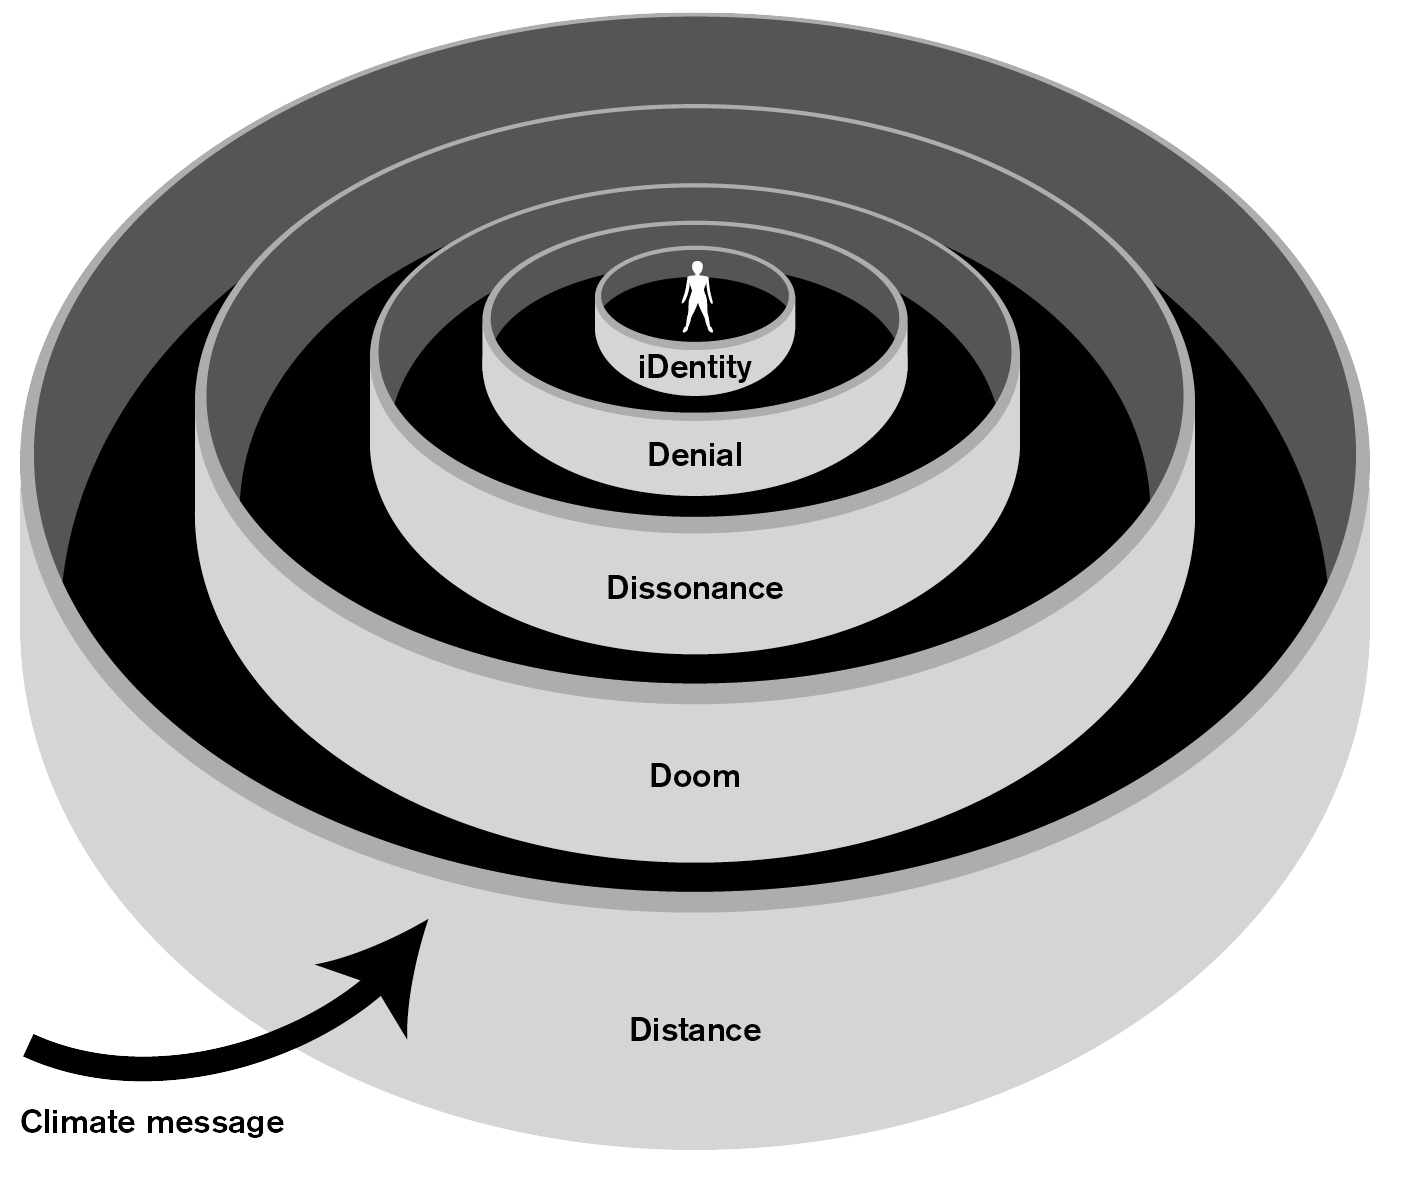
\includegraphics[width=0.9\linewidth]{figure/Analysis/5ds.png}
        	\captionsource{The five psychological barriers blocking the climate message}{What we think about when we try not to think about global warming - Per Espen Stoknes\cite{storyAboutClimateChange} (2015)}
        	\label{fig:5ds}
        \end{figure}
        
        The first barrier, \textit{Distance}, comes from e.g. a large amount of imagery of polar bears and melting ice, which can feel remote and therefore unrelatable to a majority of people\citep[p.~108]{storyAboutClimateChange}. The second barrier, \textit{Doom}, arises through fear messaging. When the climate change is framed as an inevitable disaster or the end of the world, people have a tendency to become disengaged and avoid the topic altogether\citep[p.~109]{storyAboutClimateChange}\cite{the5Ds}. \textit{Dissonance} occurs when the knowledge about e.g. the usage of fossil fuels or the meat consumption, does not match peoples behaviour. They will still drive cars and fly on vacation and eat meat. It is easy to fall in the trap of self-justification when comparing one self to other people who eat even more meat or drive and fly everywhere\citep[p.~109]{storyAboutClimateChange}\cite{the5Ds}.
        People seek refuge from fear and guilt by denying the issue. \textit{Denial} is a self-defence mechanism that happens despite the amount of information and the individual's intelligence\citep[p.~109]{storyAboutClimateChange}. \textit{Identity} is the inner most barrier. The cultural or political identity of a person can determine whether or not a person is willing to accept and adapt to climate messaging\citep[p.~109]{storyAboutClimateChange}.
        
        These barriers need to be surpassed to achieve successful communication about climate change, increase the perceived importance of it and get the public people engaged in personal climate action\cite{the5Ds}.
        
    \subsection{Climate change engagement}
        \cite{reorientingClimageChangeCommunication}\cite{vrEngagementClimateChange}
        
\section{Behavior change}
    As concluded in the previous section the problem is that the danish people's behaviour does not match the knowledge and concern they have. Therefore, research on how to change a behaviour seems appropriate.
    This section describes how games can be used to transform a player and change real world attitudes towards a subject.
    % Conclude with intermixing as a choise
    


\section{FPS}\label{sec:FPS}
\begin{quote}
    How can an immersive virtual reality transformational game incite an intent of behavioural change towards personal climate action in regards to $CO_{2}$ emissions? \todo{Tack on behavior change theory}
\end{quote}

\section{Design Requirements}\label{designReq}

\subsection{Functional design requirements}
% Make cites into refs for sub conclusions for each section.
\begin{itemize}
    \item Should incite an intent for a personal behaviour change in regards to CO$_2$ emissions.\todo{SPECIFY theory}
    \item Should implement immersive Virtual Reality to increase a sense of presence and engagement.
    \item Should lower psychological barriers, in regards to CO$_2$ emission believes.\cite{the5Ds}
    \begin{itemize}
        \item Distant
        \item Doom
        \item Dissonance
        \item Denial
        \item iDentity
    \end{itemize}
\end{itemize}


\subsection{Non-functional design requirements}
\begin{itemize}
    %Behavior change
    \item Use the transformational framework to incite behavioural change.\cite{transformationalFramework}
    %Water Consumption
    \item Use ambient exaggerated feedback(AEF) to incite a behaviour change \cite{waterConsumption}
    
    % VR
    \item Should try to maintain high Place Illusion (PI), for Immersion\citep{vrImmersion}[p.~3551].
    \item The virtual environment should be non realistic, to reduce the amount of PI breaks.
    \item Should have a virtual body to increase evidence for Plausibility Illusion(Psi), for believability \citep{vrImmersion}[p.~3553].

    %Narrative
    \item Use the player engagement process model to create engagement, incite emotions, and provide an engaging story\cite{playerEngagement}.
    %\item The narrative should challenge previous knowledge of the player, to create an engaging story.%Where is this from?
    %\item Use supportive framing that do not backfire by creating negative feelings.%Where is this from?
    
    %Embedded model
    \item It should make use of the \textit{Embedded design model} to lower psychological defences that arise when a serious social issue is communicated too directly and forthright\cite{embeddedDesignModel}.
    
    %5Ds
    \item Make the issue feel near, human, personal, and urgent to lower the distance barrier %Distance
    \item The narrative should make use of a positive story, to lower the doomsday barrier. %Doom
    \item Reduce dissonance by providing opportunities for consistent and visible action.\todo{Needs to be rephrased} %Dissonance
    \item Avoid triggering the emotional need for denial through fear, guilt, self-protection\cite{the5Ds}. %Denial
    %We need an identity requirement, if possible
    
\end{itemize}